\chapter{池化层}

池化层是当前卷积神经网络中常用组件之一,它最早见于LeNet一文,称之为Subsample。自AlexNet之后采用Pooling命名。池化层是模仿人的视觉系统对数据进行降维,用更高层次的特征表示图像\cite{RN3}。

池化层的常见操作包含以下几种:最大值池化,均值池化,随机池化,中值池化,组合池化等。

    \section{特点}
    
    在卷积神经网络过去的工作中,研究者普遍认为池化层有如下三个功效\cite{RN4}:
    
    \textbf{特征不变性} \quad 池化操作使模型更加关注\uwave{是否存在某些特征}而不是特征具体的位置。其中不变形性包括:\uwave{平移不变性、旋转不变性和尺度不变性}。
    
    \textbf{特征降维(下采样)} \quad 池化相当于在空间范围内做了维度约减,从而使模型可以抽取更加广范围的特征。同时减小了下一层的输入大小,进而减少计算量和参数个数。
    
    \textbf{在一定程度上防止过拟合} \quad 更方便优化。
    
    
    \section{分类}
    \subsection{最大值池化}
    
    最大值池化是最常见、也是用的最多的池化操作。​在前向过程,选择图像区域中的最大值作为该区域池化后的值;在后向过程中,梯度通过前向过程时的最大值反向传播,其他位置的梯度为0。前向过程的图示如图\ref{fig:11}所示。
    
    \begin{figure}[!htbp]
        \centering
        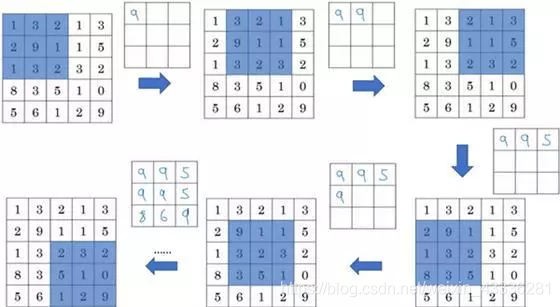
\includegraphics[width=1\textwidth]{pooling_1}
        \caption{最大值池化 \cite{RN5}}
        \label{fig:11}
    \end{figure}